\documentclass[conference]{IEEEtran}
\IEEEoverridecommandlockouts

\usepackage{cite}
\usepackage{amsmath,amssymb}
\usepackage{graphicx}
\usepackage{booktabs}
\usepackage{url}
\usepackage[hidelinks]{hyperref}
\usepackage{balance}

\graphicspath{{figures/}}

\def\BibTeX{{\rm B\kern-.05em{\sc i\kern-.025em b}\kern-.08em T\kern-.1667em\lower.7ex\hbox{E}\kern-.125emX}}

\begin{document}

\title{How Much Does Timing Matter? An Ablation of Explicit\\Phoneme Duration Modelling in Text-to-Speech}

\author{
\IEEEauthorblockN{Kunal Vats, Pushkar Jain, Tanishk Agrawal, Shaurya Sharma, Chaitanya Shekhawat}
\IEEEauthorblockA{\textit{Advanced Machine Learning --- Course Project}\\
\texttt{https://github.com/1Kunalvats9/audio\_generation}}
}

\maketitle

\begin{abstract}
Neural text-to-speech systems learn phoneme durations and spectral content jointly, which makes it
impossible to attribute output quality to either factor. We isolate the duration component by
holding the acoustic model fixed and varying only the source of the durations. Using forced
alignment on LJSpeech~1.1 we extract 949{,}856 ground-truth phone segments, train a classical
duration predictor on 905{,}833 of them, and synthesise speech twice: once from measured durations
and once from predicted ones. Gradient-boosted trees reduce duration error by 35.8\,\% relative to
a per-phone-mean baseline, from 30.61\,ms to 19.65\,ms. However, substituting predicted durations
for measured ones produced \emph{no measurable loss} of intelligibility (21.15\,\% vs 23.65\,\%
word error rate; Wilcoxon $p=0.048$, paired $t$-test $p=0.100$), whereas replacing real
spectrograms with averaged phoneme templates cost 21.17 percentage points. We conclude that at
this level of acoustic fidelity the acoustic model dominates duration accuracy by roughly a factor
of thirty, and we report the alignment and significance diagnostics that support this claim.
\end{abstract}

\begin{IEEEkeywords}
text-to-speech, forced alignment, duration modelling, gradient boosting, ablation study, speech
intelligibility
\end{IEEEkeywords}

\section{Introduction}

A text-to-speech (TTS) system must solve two coupled sub-problems. It must decide \emph{how long}
each speech sound lasts, and it must decide \emph{what each sound looks like} spectrally. The
duration problem is non-trivial: in the word \emph{cat} the vowel is substantially longer than
either consonant, and the same phone lengthens before a pause and shortens in rapid speech.

Modern end-to-end systems learn both sub-problems inside a single network. This is effective but
diagnostically opaque: when output quality is poor, the architecture offers no way to attribute
the loss to timing rather than to spectral modelling. FastSpeech~2~\cite{ren2021fastspeech2} made
duration explicit by replacing teacher-distilled durations with those produced by the Montreal
Forced Aligner (MFA)~\cite{mcauliffe2017mfa}, and routing them through a \emph{variance adaptor}.
The paper demonstrates that this improves quality overall, but does not isolate how much of that
improvement is attributable to the duration predictor specifically.

This work performs that ablation. Our contributions are:

\begin{enumerate}
\item A fully reproducible classical TTS baseline on LJSpeech~1.1 in which the acoustic model is
      deliberately held fixed, so that duration is the only free variable.
\item A duration model with 21 text-derived features and an explicitly enforced no-leakage
      guarantee, evaluated against a non-trivial baseline on a source-disjoint test split.
\item A controlled comparison (A1 vs A2) quantifying the cost of \emph{predicting} rather than
      \emph{measuring} durations, together with the significance testing needed to interpret it.
\item The negative-result finding that this cost is statistically indistinguishable from zero,
      while the acoustic model accounts for essentially all degradation.
\end{enumerate}

\section{Related Work}

\subsection{Duration in neural TTS}
FastSpeech~2~\cite{ren2021fastspeech2} is the direct antecedent of this work. Its central
methodological change was to source phoneme durations from a forced aligner rather than from a
teacher model, on the grounds that aligner durations are more accurate. Durations, pitch and
energy are predicted at inference by the variance adaptor. Our experiment targets precisely the
axis that paper introduced, and supplies the upper bound (A1, oracle durations) it does not report.

\subsection{Forced alignment}
The Montreal Forced Aligner~\cite{mcauliffe2017mfa} provides HMM/triphone alignment via Kaldi,
producing phone-level boundaries from audio and its transcript. It is the standard source of
ground-truth durations in the TTS literature and supplies our supervision signal. We treat its
output as ground truth only after validating it (Section~\ref{sec:align}).

\subsection{Neural vocoding}
HiFi-GAN~\cite{kong2020hifigan} reconstructs waveforms from mel spectrograms with high fidelity at
low computational cost. We use a frozen pre-trained checkpoint so that the vocoder contributes an
identical, constant transformation to every system under comparison.

\subsection{Diffusion-based speech generation}
Grad-TTS~\cite{popov2021gradtts} applies a score-based diffusion process in mel space, and
AudioLDM~\cite{liu2023audioldm} operates in a learned latent space. These represent the natural
successor to the template-based acoustic model used here; Section~\ref{sec:future} explains why
our results point towards this component rather than towards better duration modelling.

\subsection{Evaluation by automatic speech recognition}
Human mean-opinion-score studies are the standard for naturalness but require a listening panel.
Using an ASR system as a proxy listener gives a reproducible, automatic measure of
\emph{intelligibility}. We use Whisper~\cite{radford2023whisper} in its \texttt{small.en}
configuration. We note explicitly that this measures intelligibility and not naturalness, a
limitation revisited in Section~\ref{sec:limits}.

\section{Dataset and Exploratory Analysis}

\subsection{Corpus}
LJSpeech~1.1~\cite{ljspeech2017} comprises 13{,}100 utterances read by a single female speaker
from seven public-domain non-fiction texts, sampled at 22{,}050\,Hz, 16-bit mono, totalling
23.92 hours.

We verified the corpus rather than trusting its documentation. All 13{,}100 metadata rows have
unique identifiers with exactly one matching waveform each (zero missing, zero extra); every file
is 22{,}050\,Hz mono. Clip length ranges from 1.11\,s to 10.10\,s with a median of 6.76\,s,
corresponding to 96--870 mel frames. Fig.~\ref{fig:dataset} shows the distributions.

\begin{figure}[t]
\centering
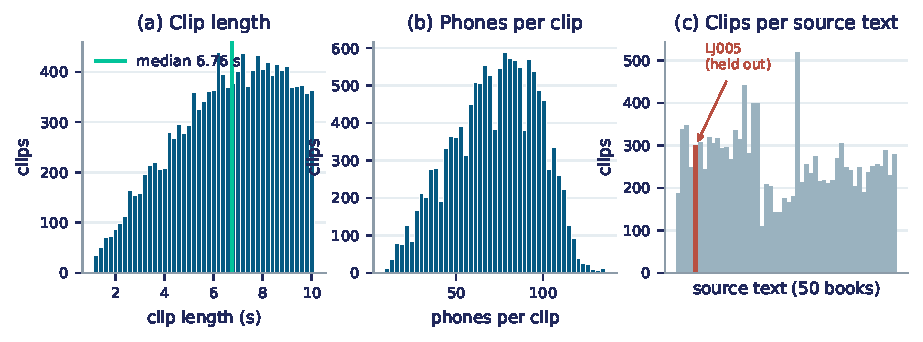
\includegraphics[width=\columnwidth]{fig_dataset.pdf}
\caption{Corpus statistics. (a) Clip length. (b) Phones per clip after alignment. (c) Clips per
source text; the held-out book \texttt{LJ005} is highlighted.}
\label{fig:dataset}
\end{figure}

\subsection{Text normalisation}
The aligner requires orthographic text reducible to dictionary entries, so numerals and symbols
must be expanded. Comparing the raw and supplied-normalised transcripts showed they differ in
1{,}505 rows (11.5\,\%), which determined that the normalised column is the correct source. After
our cleaning, \textbf{zero digits and zero non-ASCII characters} remain across all 13{,}100 rows.

Three ambiguities were resolved by inspecting the data rather than by assumption. All 16
occurrences of \texttt{St.} are place names, with a single genuine \emph{Street} case
(\texttt{LJ007-0230}), so the many-case expansion to \emph{saint} was adopted. The sole
\texttt{ft.} occurrence is \emph{Dallas-Ft.\ Worth}, giving \emph{fort}. The 17 occurrences of
\texttt{messrs.} were deliberately left unexpanded, since the MFA dictionary already contains
\texttt{messrs} as \texttt{M EH1 S ER0 Z}, matching the speaker's realisation.

\subsection{Partitioning}
With a single speaker, speaker-disjoint evaluation is impossible. We therefore hold out whole
source texts: all 299 clips of book \texttt{LJ005} form the test set, guaranteeing that no test
sentence shares its source document with any training sentence. This yields 12{,}501 training,
300 validation and 299 test clips; a fixed 100-clip subset (\texttt{test\_100}) is used for
synthesis and listening evaluation. All partitioning uses seed 42.

\section{Method}

\subsection{Forced alignment and its validation}
\label{sec:align}
MFA was run with the \texttt{english\_us\_arpa} acoustic model and dictionary. 366 words in
LJSpeech are absent from that dictionary (proper nouns, compounds, acronyms such as \emph{FBI}),
affecting 1{,}179 clips; without pronunciations these clips would be discarded. We generated a
supplementary dictionary so that \textbf{all 13{,}100 clips aligned with none excluded}, yielding
\textbf{949{,}856 phone segments} over 70 labels (39 ARPAbet phones with stress digits, plus
silence).

Because every downstream result depends on these boundaries, we validated them with a test that
includes its own control. At each speech--silence transition, frame energy should change in the
expected direction. It does so for \textbf{94.6\,\%} of 1{,}878 boundaries. Repeating the test
with every boundary displaced by five frames ($\approx$58\,ms) gives \textbf{53.7\,\%}, i.e.\
chance. A misaligned system would score equivalently on both; the separation is therefore evidence
that the boundaries track real acoustic events.

As an independent check, the measured durations reproduce phonetic regularities we did not encode.
\texttt{DH} is the shortest phone at 35\,ms, diphthongs are longest, and stressed vowels average
108\,ms against 67\,ms for unstressed vowels (Fig.~\ref{fig:durations}).

\begin{figure}[t]
\centering
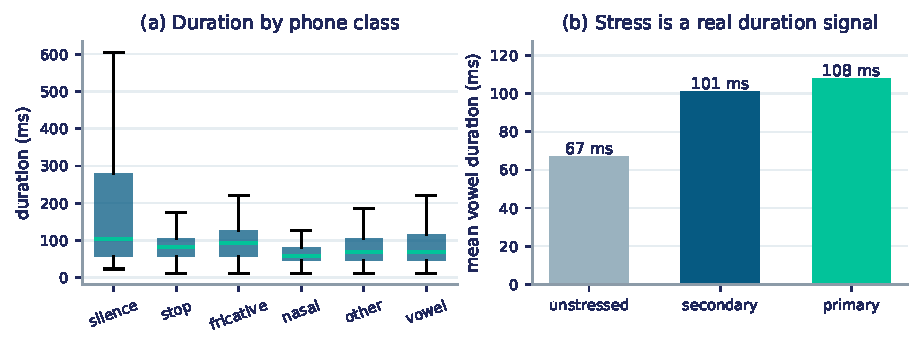
\includegraphics[width=\columnwidth]{fig_durations.pdf}
\caption{Durations recovered by forced alignment. (a) By phone class. (b) The stress effect, which
motivates retaining ARPAbet stress digits as distinct labels.}
\label{fig:durations}
\end{figure}

\subsection{Acoustic representation}
Audio is converted to 80-band log-mel spectrograms with a 1024-sample window and a 256-sample hop,
giving a frame period of $256/22050 = 11.61$\,ms. All durations in this work are expressed in
these frames.

The vocoder checkpoint was trained with a specific mel convention (amplitude rather than power
spectra, Slaney normalisation and mel scale, natural logarithm after clamping at $10^{-5}$). A
mismatch here degrades audio in ways that are difficult to detect by ear, so we verified our
implementation against the reference implementation numerically and obtained a mean absolute
difference of $0.000000$ before proceeding.

\subsection{Feature engineering}
\label{sec:features}
The duration model predicts the length of each phone from 21 features, \emph{all derived from
text alone}. Five are categorical: the phone identity (retaining its stress digit), the preceding
and following phone (with boundary tokens at clip edges, computed within clips so context never
crosses an utterance), a six-way phone class, and the stress level. Sixteen are numeric: position
within the word, word length, whether the phone is word-initial or word-final, position of the
word within the utterance, position of the phone within the utterance, counts of phones and words,
silence indicators for the phone and its neighbours, and the distance in phones to the nearest
silence on each side.

The last pair encodes \emph{pre-pausal lengthening}, the documented tendency of segments to
lengthen before a pause. Fig.~\ref{fig:importance} confirms the model exploits it.

\textbf{Leakage control.} The most predictive available feature would be the utterance's true
total length divided by its phone count --- an excellent tempo estimate, and unavailable at
synthesis time. We exclude every feature derived from true duration and enforce this with a unit
test that multiplies all durations by three and asserts the resulting feature matrix is
bit-identical. Notably this costs nothing: synthesis rescales predicted durations to the target
utterance length, so any utterance-level tempo scalar is divided out again. The model need only
recover durations \emph{relative to one another} within an utterance.

\subsection{Duration models}
All models regress $\log(\textrm{frames})$ rather than frames. Durations are strongly right-skewed
--- the median phone is 7 frames while silences reach 481 --- so a squared-error objective on raw
counts would allocate most capacity to a few long pauses. This matches the parameterisation used
by FastSpeech~2's duration predictor.

Three models are compared, fitted on \texttt{train}, selected on \texttt{val} and reported once on
\texttt{test}:

\begin{itemize}
\item \textbf{Per-phone mean.} The mean log-duration of each phone type, with a global fallback.
      A non-trivial baseline that any contextual model must beat.
\item \textbf{Ridge regression.} One-hot encoded categoricals and standardised numerics; the
      penalty $\alpha$ was selected on validation from $\{0.1, 1, 10, 100\}$.
\item \textbf{Gradient-boosted trees.} Histogram-based boosting with native categorical splits.
      Training halts on validation plateau, converging at 1{,}052 iterations.
\end{itemize}

\subsection{Synthesis}
To hold the acoustic model constant we use \emph{phoneme templates}. For each of the 70 phones,
every training occurrence is divided into three equal temporal states and averaged across
occurrences, producing one fixed $80 \times 3$ matrix per phone. An utterance is synthesised by
stretching each phone's three states to its assigned duration, concatenating, and passing the
result to the frozen HiFi-GAN vocoder.

Predicted durations are emitted as unrounded reals and converted to integers that sum exactly to
the target frame count, with every phone constrained to at least one frame.

\section{Experimental Setup}

Four systems are compared on the same 100 utterances, differing in exactly one component each:

\begin{table}[t]
\caption{The four systems. Each row changes one component relative to the row above.}
\label{tab:systems}
\centering
\begin{tabular}{llp{3.5cm}}
\toprule
\textbf{System} & \textbf{Spectrogram} & \textbf{Durations} \\
\midrule
R0 & --- (original audio) & --- \\
R1 & real, from audio & real \\
A1 & phoneme templates & \textbf{measured} (oracle) \\
A2 & phoneme templates & \textbf{predicted} \\
\bottomrule
\end{tabular}
\end{table}

The contrast of interest is A1 vs A2, which differ \emph{only} in the source of the durations;
templates, vocoder and target utterance length are identical. R0 establishes the error floor of
the measuring instrument and R1 isolates the vocoder's contribution.

Intelligibility is measured as word error rate (WER) and character error rate (CER) between the
reference transcript and Whisper's hypothesis, with both strings passed through Whisper's
\texttt{EnglishTextNormalizer} so that punctuation and orthographic variation are not scored.

\section{Results}

\subsection{Duration modelling}
Table~\ref{tab:duration} reports performance on the 299 held-out utterances. Gradient-boosted
trees reduce error by \textbf{35.8\,\%} relative to the per-phone-mean baseline. The ordering
(baseline $>$ ridge $>$ trees) is the expected one; an inversion would have indicated leakage or a
defect. Validation and test figures agree closely for the selected model (1.702 vs 1.693 frames),
indicating that selection did not overfit.

Every metric is reported twice, with and without silence. Silence constitutes only 5.3\,\% of
segments but averages 14.6 frames against 7.4 for speech segments, with a maximum of 481; it
therefore dominates an aggregate error figure. The silence-excluded column is the more faithful
measure of learned phone duration, while the inclusive column is what synthesis actually consumes.

\begin{table}[t]
\caption{Duration prediction on the held-out book (299 utterances, 22{,}696 phones).
One frame is 11.61\,ms.}
\label{tab:duration}
\centering
\begin{tabular}{lrrrr}
\toprule
\textbf{Model} & \textbf{MAE} & \textbf{MAE} & \textbf{MAE excl.} & \textbf{RMSE} \\
               & (frames) & (ms) & sil.\ (ms) & (frames) \\
\midrule
Per-phone mean  & 2.637 & 30.61 & 26.88 & 4.34 \\
Ridge           & 2.338 & 27.14 & 23.31 & 3.93 \\
\textbf{Boosted trees} & \textbf{1.693} & \textbf{19.65} & \textbf{16.84} & \textbf{3.08} \\
\bottomrule
\end{tabular}
\end{table}

Fig.~\ref{fig:importance} gives permutation importance on the validation split. Phone identity
dominates, as expected, but the contextual features contribute materially --- in particular the
distance-to-silence pair, confirming that the model recovers pre-pausal lengthening from data.

\begin{figure}[t]
\centering
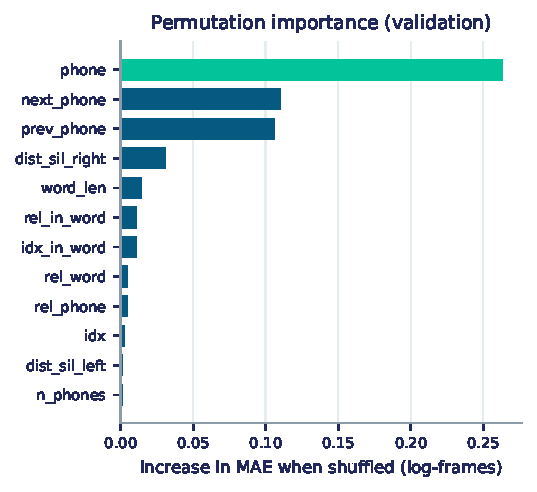
\includegraphics[width=0.84\columnwidth]{fig_importance.pdf}
\caption{Permutation importance of the twelve strongest features, measured as the increase in
validation MAE when a feature is shuffled.}
\label{fig:importance}
\end{figure}

\subsection{Intelligibility}
Table~\ref{tab:wer} reports WER and CER for all four systems.

\begin{table}[t]
\caption{Intelligibility, 100 utterances per system, Whisper \texttt{small.en}.}
\label{tab:wer}
\centering
\begin{tabular}{llrr}
\toprule
\textbf{System} & \textbf{Description} & \textbf{WER} & \textbf{CER} \\
\midrule
R0 & original recording          & 1.85\,\%  & 0.71\,\%  \\
R1 & real mel $\rightarrow$ vocoder & 2.48\,\%  & 0.95\,\%  \\
A1 & templates + measured durations & 23.65\,\% & 11.83\,\% \\
A2 & templates + predicted durations & 21.15\,\% & 10.02\,\% \\
\bottomrule
\end{tabular}
\end{table}

Decomposing the chain attributes the degradation to specific components:

\begin{itemize}
\item \textbf{R0 $\rightarrow$ R1: $+0.63$ pp.} The mel representation and the vocoder are
      nearly lossless. R0's own non-zero floor is partly an artefact of reference normalisation:
      three of its ten worst utterances are cases where the reference reads \emph{``george the
      4th''} and Whisper outputs \emph{``george iv''}.
\item \textbf{R1 $\rightarrow$ A1: $+21.17$ pp.} Replacing real spectrograms with averaged
      templates accounts for essentially all loss --- roughly 34 times the vocoder's cost.
\item \textbf{A1 $\rightarrow$ A2: $-2.50$ pp.} Predicting durations rather than measuring them
      did not degrade intelligibility.
\end{itemize}

\subsection{Statistical analysis of the A1--A2 contrast}
\label{sec:stats}
The sign of the A1--A2 difference is opposite to our expectation, so we tested it rather than
reporting it at face value. On the same 100 utterances, A2 is better on 40, worse on 30 and tied
on 30. A Wilcoxon signed-rank test gives $p=0.048$; a paired $t$-test gives $p=0.100$.

One test crosses the conventional threshold and the other does not. \textbf{We therefore do not
claim that predicted durations are superior to measured ones.} The defensible conclusion is the
weaker and more interesting one:

\begin{quote}
At this level of acoustic fidelity, duration prediction error of 19.65\,ms has no measurable
effect on intelligibility. The acoustic model, not the duration model, is the binding constraint.
\end{quote}

\subsection{Why is A2 not worse? A partial explanation}
We investigated the mechanism and report an unconfirmed hypothesis rather than a conclusion.

Our first conjecture --- that regression toward the mean smooths the predictions --- is
\emph{false}: predicted durations are more dispersed than measured ones ($\sigma = 7.04$ vs
$5.01$ frames), partly because the rescaling step assigns residual frames to the longest segment,
producing phones of up to 154 frames against a true maximum of 76.

The surviving hypothesis concerns very short segments. A three-state template cannot be rendered
in a single frame. Measured durations place 3.5\,\% of segments at two frames or fewer, whereas
predicted durations place only 0.8\,\% there. Across utterances, the more short segments A2
eliminated, the more it improved ($r = +0.227$, $p = 0.023$). However, A1's own error does not
track its short-segment fraction ($r = +0.014$, $p = 0.89$), so the mechanism is \textbf{not
established}; we report it as a direction for further work.

\section{Discussion}

\subsection{Limitations}
\label{sec:limits}
\textbf{A2 receives oracle utterance length.} Predicted durations are rescaled to the true total
length, information a deployed system would not possess. Our comparison therefore isolates the
\emph{relative} distribution of durations, not total-length prediction, and A2 is not a fully
autonomous system. We adopted this to ensure both systems present the vocoder with
identically-sized inputs.

\textbf{Intelligibility is not naturalness.} WER cannot detect prosodic flatness. Given an
acoustic model consisting of per-phone averages, we expect the output to be intelligible yet
clearly synthetic, and our evaluation is blind to the latter.

\textbf{A single speaker.} Speaker generalisation cannot be assessed; the source-disjoint split is
the strongest available substitute.

\textbf{Deliberately weak acoustic model.} Phoneme templates discard coarticulation and all
prosody beyond duration. This is required by the experimental design but bounds the attainable
quality of A1 and A2.

\subsection{Implications for FastSpeech~2}
Our results support the premise that forced-aligner durations are accurate, but suggest that under
a weak acoustic model, improvements to the duration predictor yield little intelligibility gain.
The value of the variance adaptor is more plausibly in naturalness, which our instrument cannot
measure --- a hypothesis a listening study could test directly.

\subsection{Engineering notes}
The repository carries 170 automated tests, including tests that guard shared numerical contracts:
the frame-count formula, the mel convention against the vocoder's reference implementation, and
the no-leakage property of Section~\ref{sec:features}. Three substantive defects were found only
by executing the full pipeline rather than by inspection: a residual-distribution error that
corrupted 27 of 299 utterances, a type error that aborted synthesis, and an empty-slice
\texttt{NaN} that silently invalidated 61 of 70 templates. Each is now covered by a regression
test.

\section{Conclusion and Future Work}
\label{sec:future}

We isolated the duration component of a TTS pipeline by holding the acoustic model fixed.
Gradient-boosted trees on 21 text-derived features reduced duration error by 35.8\,\% over a
per-phone-mean baseline. Substituting those predictions for oracle durations produced no
measurable intelligibility loss, while the averaged-template acoustic model accounted for 21.17
percentage points of degradation.

The practical implication is that further effort belongs in the acoustic model rather than in
duration modelling. Diffusion-based generators~\cite{popov2021gradtts, liu2023audioldm} are the
natural replacement, and the alignment and duration infrastructure developed here supplies exactly
the conditioning signal such a model requires. Three concrete next steps follow: predict total
utterance length so that A2 becomes autonomous; distribute the rescaling residual proportionally
rather than onto a single segment; and conduct a human listening study to measure the naturalness
dimension that WER cannot observe.

\section*{Contributions}

\textbf{Kunal Vats} --- corpus preparation, text normalisation, partitioning, shared configuration;
duration model (with Pushkar Jain).
\textbf{Pushkar Jain} --- duration model: feature construction, model comparison, error analysis
(with Kunal Vats).
\textbf{Tanishk Agrawal} --- forced alignment, out-of-vocabulary dictionary, alignment validation.
\textbf{Shaurya Sharma} --- mel extraction, phoneme templates, vocoder integration, synthesis.
\textbf{Chaitanya Shekhawat} --- ASR evaluation harness, results aggregation, failure analysis.

\balance
\bibliographystyle{IEEEtran}
\bibliography{refs}

\end{document}
